\subsubsection{Tổng quan}
Sơ đồ use-case \textbf{màn hình chính}:
\begin{figure}[H]
    \centering
    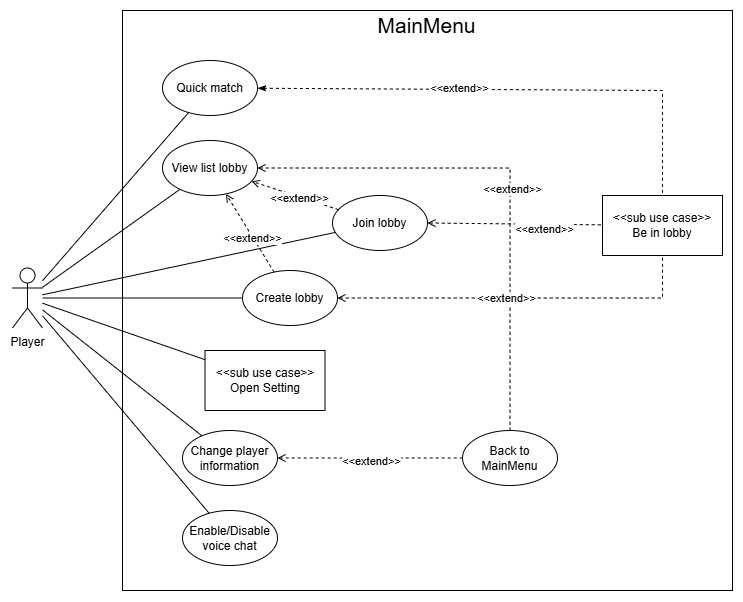
\includegraphics[width=0.75\linewidth]{4.Đặc tả chi tiết các lược đồ/Use-case/images/MainMenu.png}
    \caption{Use-case mô tả màn hình chính}
    \label{fig:placeholder}
\end{figure}

Người chơi có thể chỉnh sửa thông tin cá nhân, vào phòng chơi bằng cách chọn phòng hoặc tạo phòng hoặc vào phòng nhanh (quick match). Cùng với đó còn có các chức năng khác người dùng có thể thực hiện trong các use-case phụ trong use-case màn hình chính, cụ thể use-case bao gồm các use-case phụ sau:
\begin{itemize}
    \item \textbf{Mở cài đặt}: Tại đây sẽ dẫn người chơi vào use-case Settings, use-case này mô tả các hoạt động có thể thực hiện được khi mở cài đặt.
    \item \textbf{Trong phòng}: tại đây  sẽ dẫn người chơi vào use-case In Lobby, use-case này mô tả các hoạt động có thể thực hiện được khi vào đã vào trong lobby.
\end{itemize}